\documentclass[11pt]{article}
\usepackage[margin=0.8in]{geometry}
\usepackage{graphicx}
\usepackage{booktabs}
\usepackage{longtable}
\usepackage{amsmath}
\usepackage{hyperref}
\usepackage{xcolor}
\usepackage{enumitem}
\hypersetup{colorlinks=true,linkcolor=black,urlcolor=blue}
\setlist{nosep}
\definecolor{accent}{HTML}{8F2D20}
\newcommand{\code}[1]{\texttt{#1}}
\title{\textbf{Eta Carinae 18 Micron Homunculus Reconstruction}\\\large Session Summary, Methodology, Algorithms, and Products}
\author{}
\date{14 September 2026}
\begin{document}
\maketitle
\begin{center}
\color{accent}\textbf{Provisional figure-derived morphology and flux-scale estimate; not archival photometry or an astrometric solution}
\end{center}

\section{Objective and Source Material}
The objective was to reconstruct a continuous two-dimensional 18 micron surface-brightness map of the Eta Carinae Homunculus. Smith (2003) Figure 3 supplies high-resolution color morphology but no direct flux scale; Figure 1e supplies published 18 micron contours in Jy arcsec$^{-2}$. The reconstruction combines these sources and integrates the result across the minor axis to produce power per unit angle along the major axis in Jy arcsec$^{-1}$.

Figure 3 maps 18.0, 12.5, and 8.8 microns to red, green, and blue. The 22 published Figure 1e levels span 30--3200 Jy arcsec$^{-2}$. Embedded PDF rasters xref 35 and 69 were extracted, and vector drawings 212--252 supplied the Figure 1e contour segments. Segments were preserved independently to avoid artificial connectors.

\section{Image Preparation}
The unique intersecting long vector lines in Figure 1e locate the stellar cross. The embedded Figure 1e raster has a negative vertical PDF placement transform, so its extracted rows are reversed before raster sampling and side-by-side display; this aligns it with the Figure 1e vector coordinates and Figure 3. In Figure 3, central dark row and column projections locate the stellar marker at pixel $(344.5,350.5)$. The printed marker was removed with a compact mask and Telea inpainting while retaining the central region in the scientific footprint.

The native Figure 3 footprint was formed from HSV saturation/value thresholds, morphological closing, the component nearest the star, dilation, and hole filling. Annotation regions were excluded. The final grid is $676\times680$ pixels and remains unwarped.

\section{Spatial Calibration}
The original nominal 13 arcsec full-frame interpretation compressed the visible Homunculus to about $\pm4.5$ arcsec and was rejected. Figure 1e labeled ticks give 21.14 PDF units per 2 arcsec, or 0.0610047292 arcsec pixel$^{-1}$ in its raster.

Figure 3 tick positions are measured from all four raster borders. The detector converts to grayscale, computes perpendicular-stroke contrast in narrow border strips, searches a 36--41 pixel period/phase comb, refines local maxima, and fits a regular sequence. Opposing edges are combined separately by axis.

\begin{center}
\begin{tabular}{lrr}
\toprule
Edge & Spacing (pixels/tick) & RMS residual (pixels)\\
\midrule
Top & 38.7662 & 0.490\\
Bottom & 38.7574 & 0.298\\
Left & 38.2559 & 0.330\\
Right & 38.2559 & 0.305\\
\bottomrule
\end{tabular}
\end{center}

Assuming 1 arcsec per regular unlabeled Figure 3 interval gives $CDELT1=+0.0257999733$ and $CDELT2=-0.0261397709$ arcsec pixel$^{-1}$. Their difference is retained. The star-anchored Figure 1e-to-Figure 3 contour scales are 2.364527 in X and 2.333790 in Y, with zero rotation. The 1 arcsec interval is an explicit inference, not independent astrometry; 0.5 and 2 arcsec alternatives imply fields of about 8.8 and 35.2 arcsec.

\begin{center}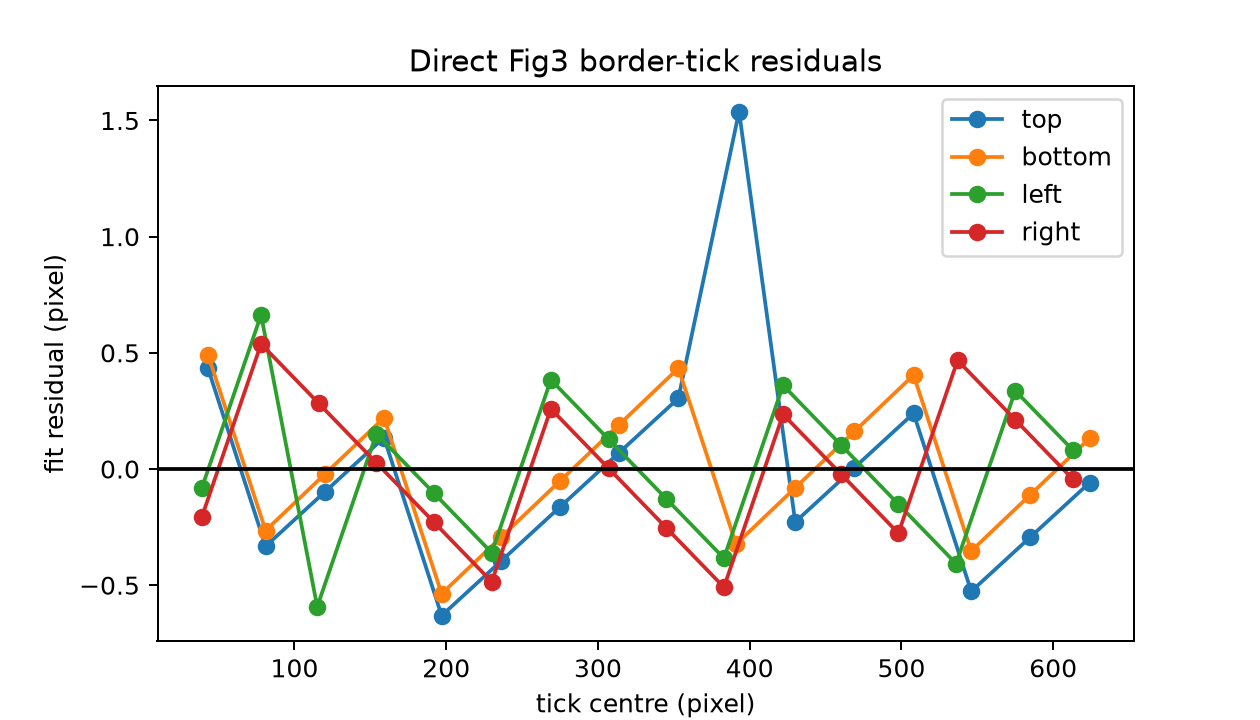
\includegraphics[width=0.72\textwidth]{outputs/diag_tick_residuals.png}\end{center}

\section{Morphology and Flux Calibration}
Grayscale samples normal to Figure 1e vector segments were grouped into the 22 published levels by contiguous dynamic programming with a monotonicity penalty. Red, luminance, and constrained RGB predictors were compared by leave-one-level-out cross-validation. RMSE values were 256.61, 288.64, and 256.61 Jy arcsec$^{-2}$, respectively; the optimal constrained weights were $[1,0,0]$. The physically appropriate red-only model was retained.

Contour red values and assigned flux levels were fitted with a pooled-adjacent-violators isotonic relation and piecewise-linear interpolation. Emission below 30 Jy arcsec$^{-2}$ is unsupported. Values above the highest effective anchor, 2253.08 Jy arcsec$^{-2}$, are held there and flagged as lower bounds. The 2500 and 3200 Jy arcsec$^{-2}$ contours are therefore unavailable.

The native angular center bounds are X $[-8.8881,8.6301]$ arcsec and Y $[-8.4824,9.1620]$ arcsec. No science map or mask is spatially resampled.

\begin{center}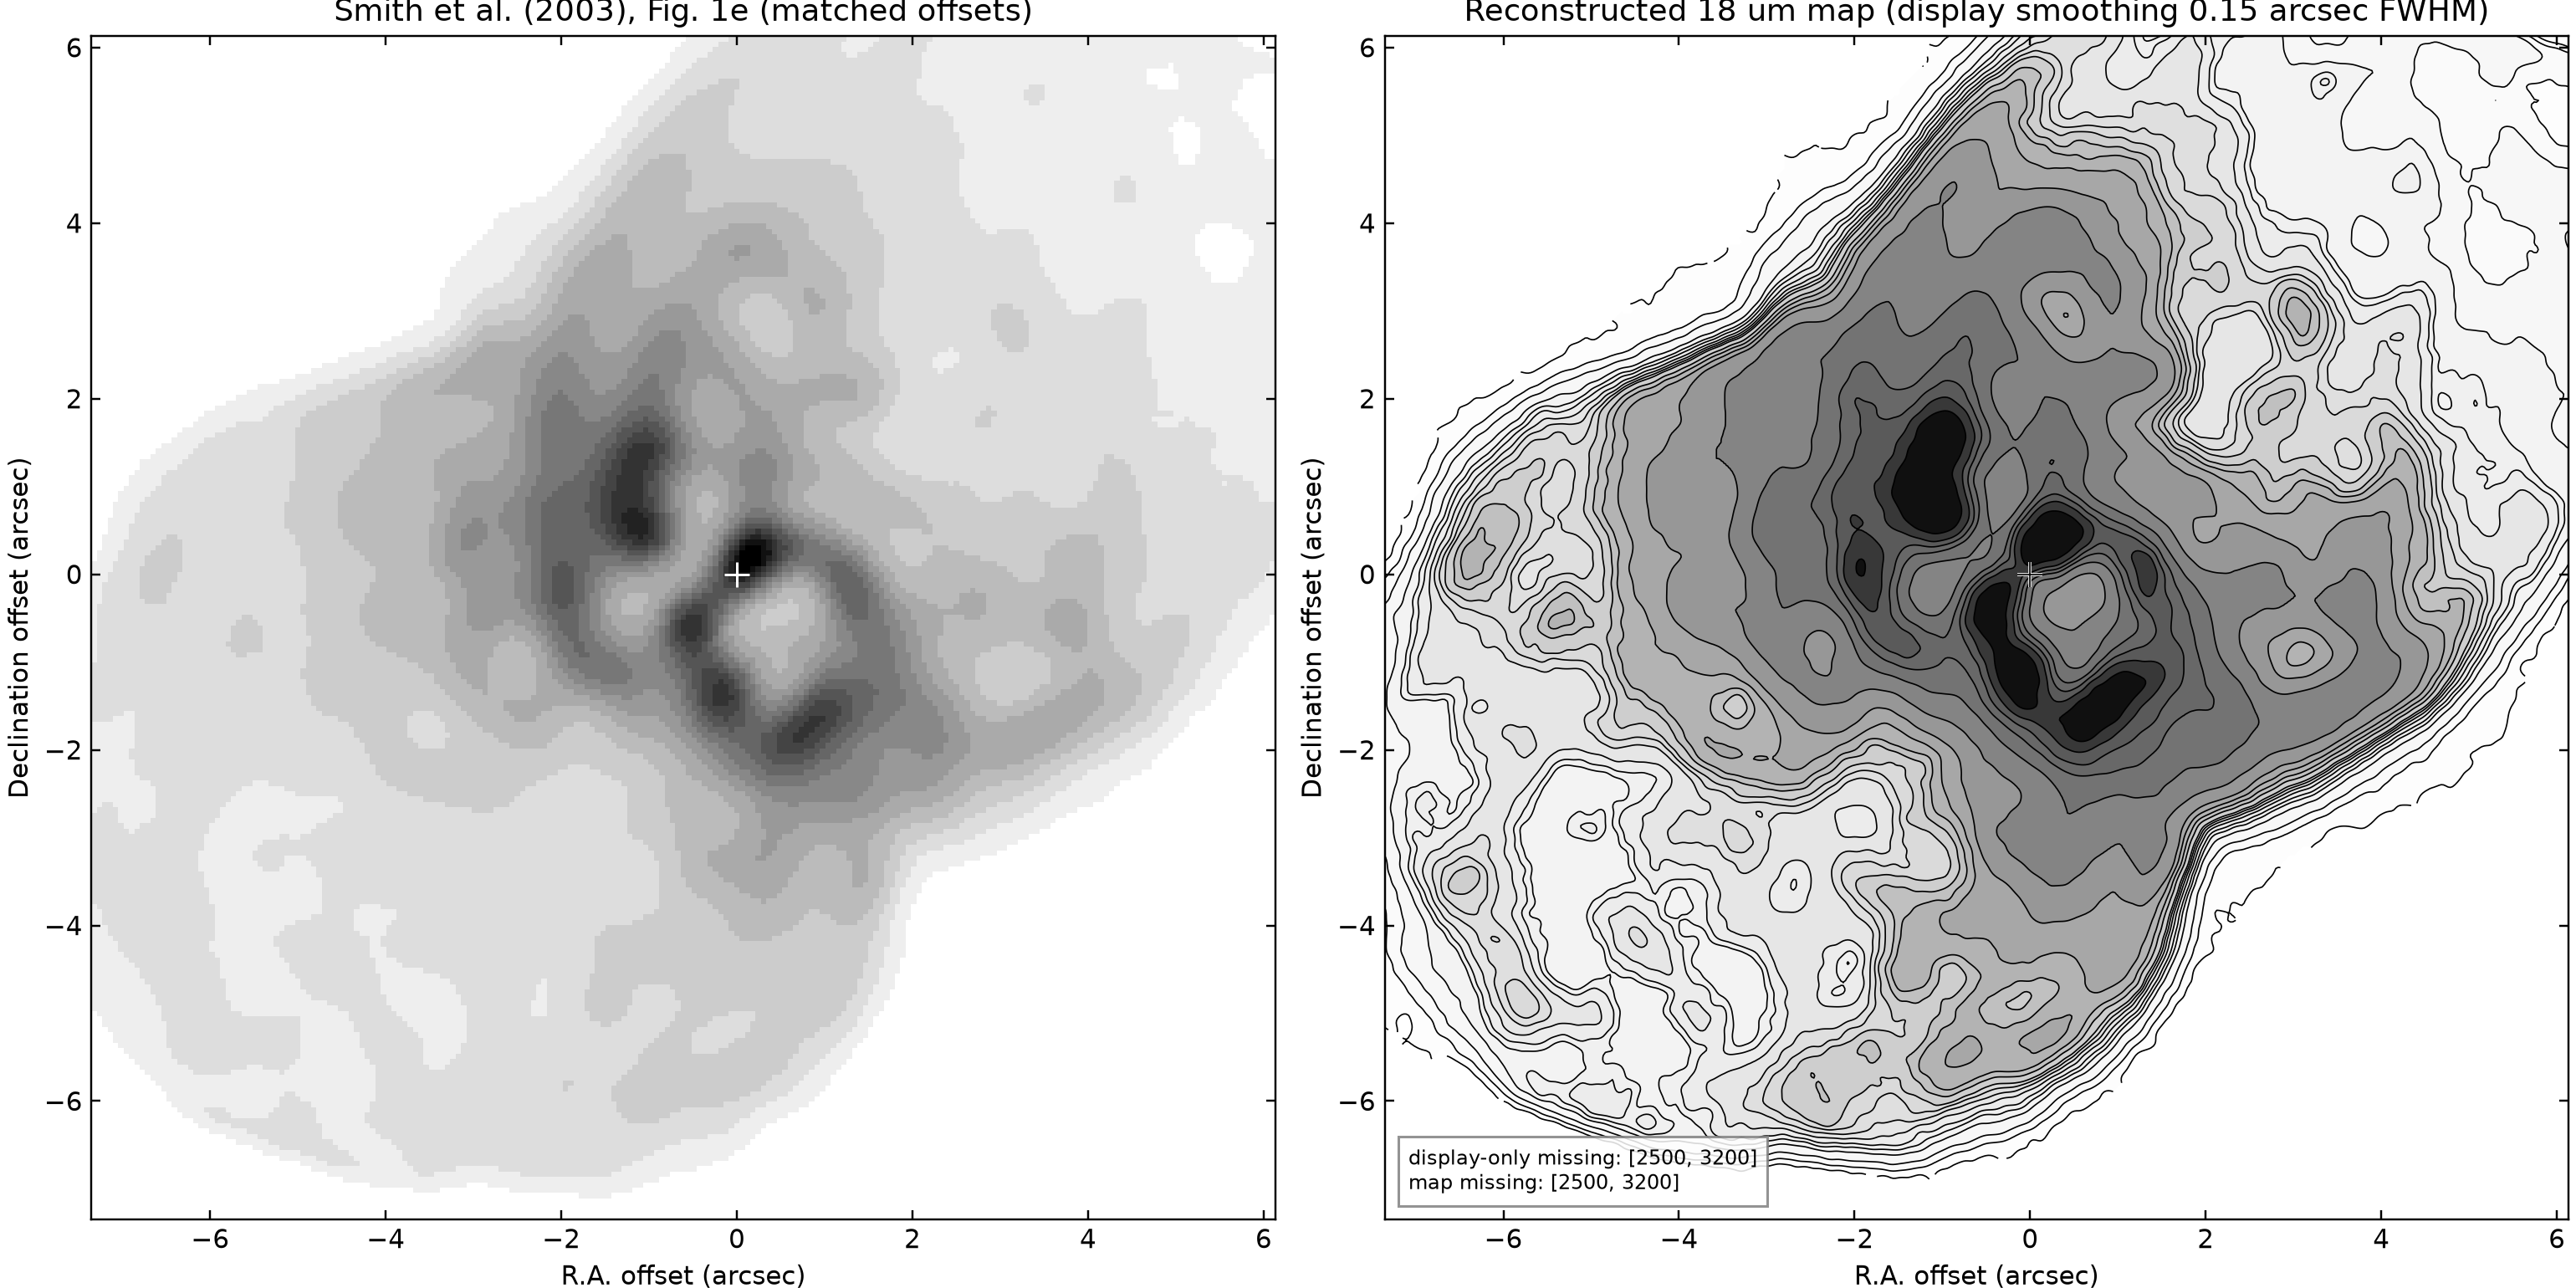
\includegraphics[width=\textwidth]{outputs/comparison_fig1e_reconstruction.png}\end{center}

\section{Visualization and Major-Axis Profile}
Contours use all published levels supported by the map. Mask-normalized 0.15 arcsec FWHM smoothing is display-only and never alters FITS or NPZ arrays.

For the one-dimensional profile, the major axis is assigned $PA=132^\circ$ east of north, positive southeast. This standard orientation is adopted, not fitted. For pixel offsets $(x,y)$,
\[
s=-x\sin(PA)+y\cos(PA),
\]
The displayed horizontal offset increases to the right while astronomical east increases to the left, hence the negative $x$ term. Native pixels are accumulated in 0.1 arcsec bins. With intensity $I_i$, pixel area $A_{\rm pix}$, and bin width $\Delta s$,
\[
P(s)=\frac{\sum_i I_i A_{\rm pix}}{\Delta s}, \qquad
\sum P(s)\Delta s=\sum I_iA_{\rm pix}.
\]
Thus $P$ has units Jy arcsec$^{-1}$. The integrated profile flux is 99550.08 Jy. It remains provisional because the source map is figure-derived and sub-30 Jy arcsec$^{-2}$ emission is unconstrained.

\begin{center}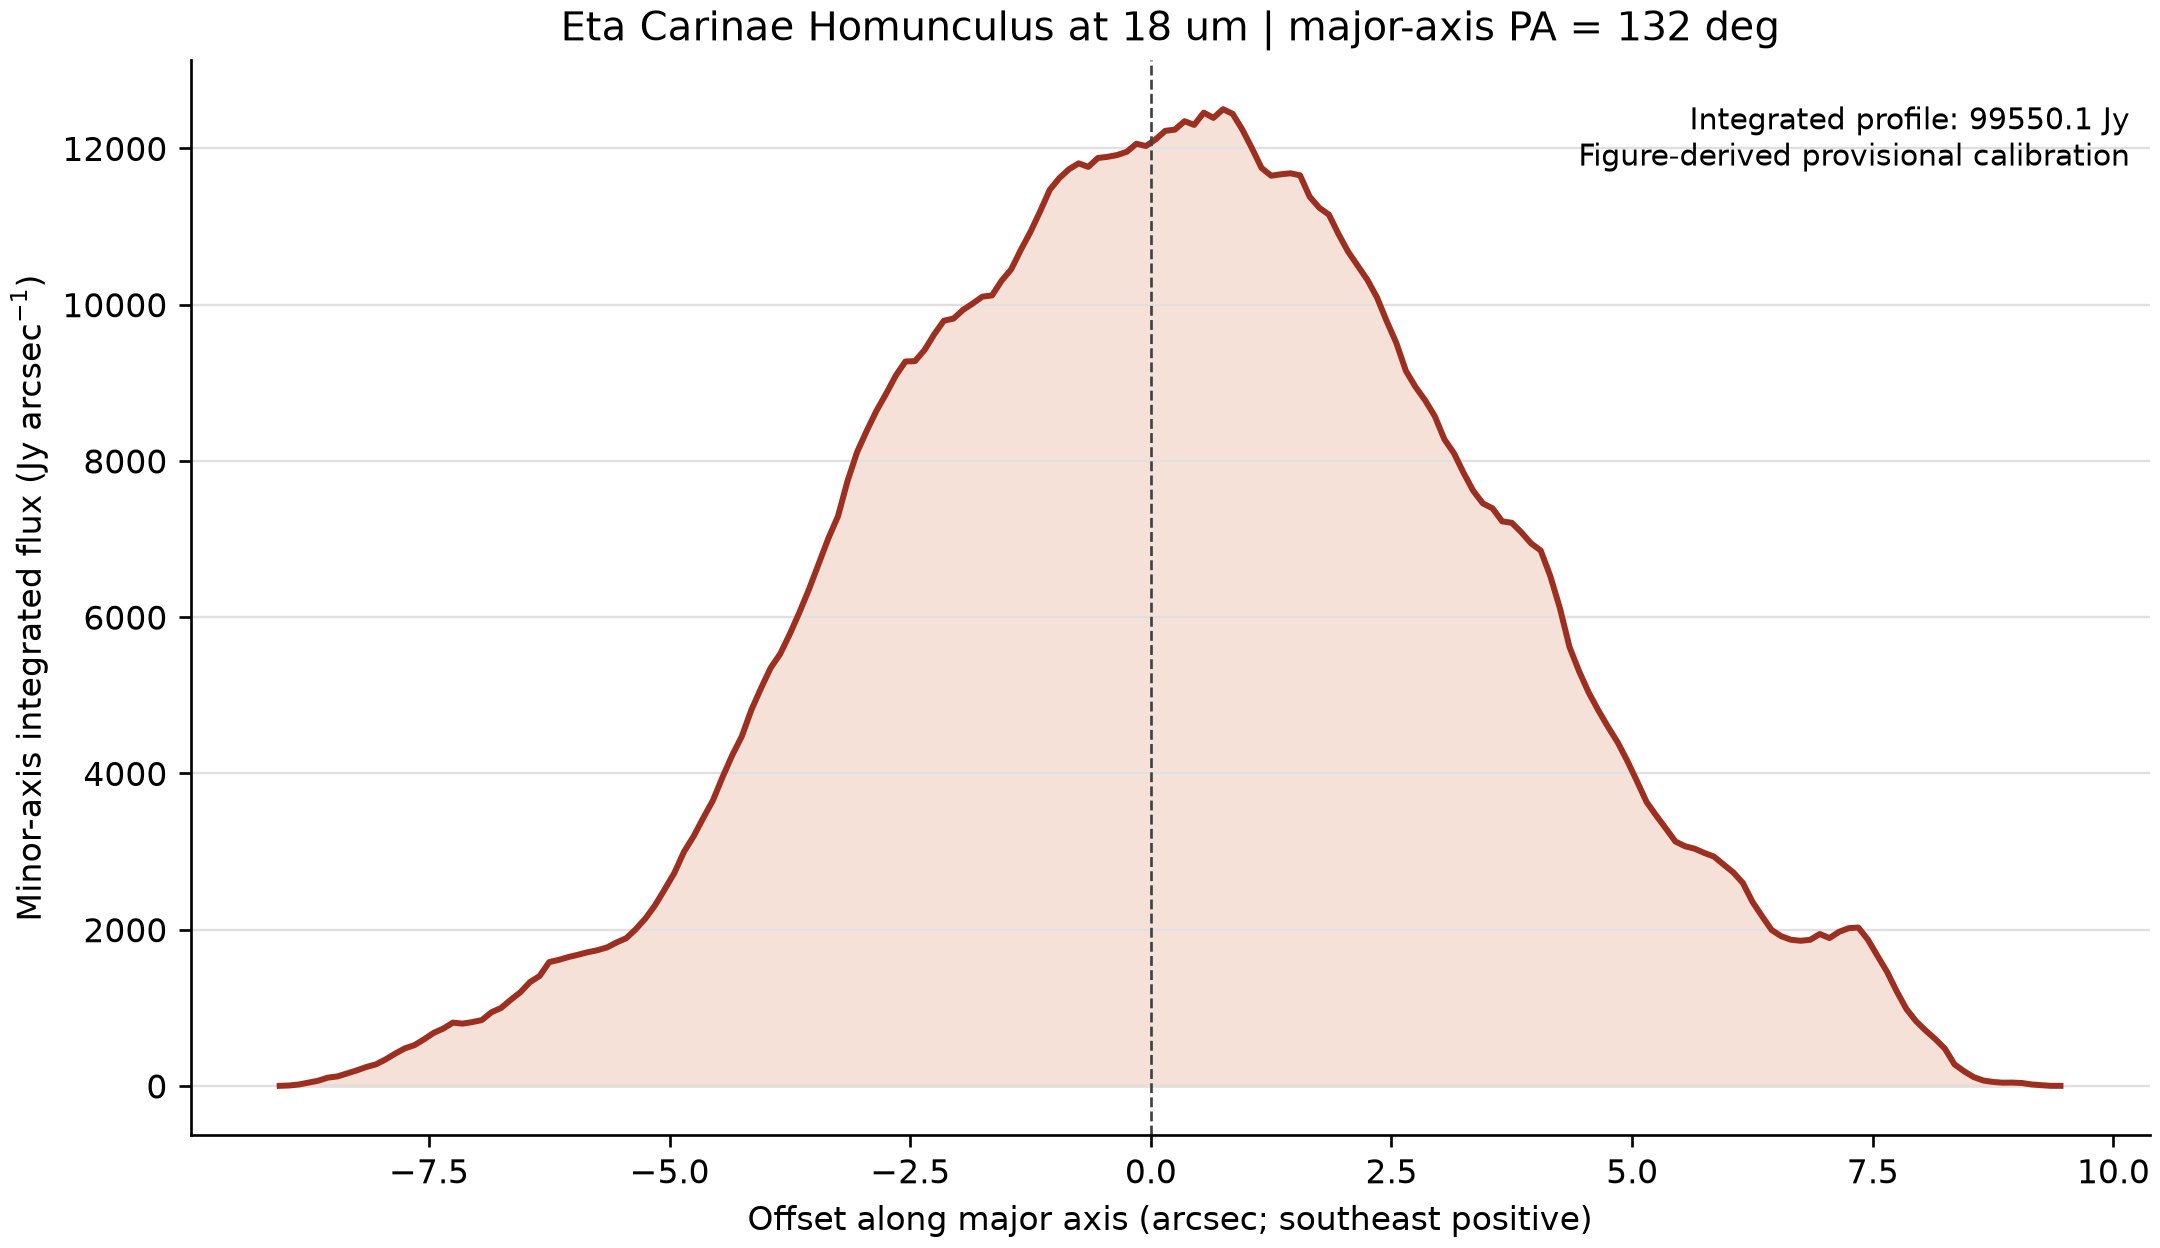
\includegraphics[width=0.95\textwidth]{outputs/i18_major_axis_profile.png}\end{center}

\section{Validation}
Raster evidence is used on four borders; opposing-edge spacings agree to 0.0088 pixel in X and effectively exactly in Y. Residual RMS is 0.30--0.49 pixel. The star maps exactly to angular zero. FITS and NPZ maps are exactly equal at native dimensions, normalized weights sum to one, and the profile conserves integrated flux. The test suite reports one passing test; warnings are PyMuPDF/SWIG deprecations. Independent final verification returned PASS for the corrected calibration and honest provisional labeling.

\section{Files}
\begin{itemize}
\item \textbf{Scripts:} \path{reconstruct_homunculus_map.py}, \path{plot_reconstructed_contours.py}, \path{plot_major_axis_profile.py}, \path{tests/test_reconstruction.py}, and \path{requirements.txt}.
\item \textbf{Maps and profiles:} \path{outputs/i18_map.fits}, \path{outputs/i18_map.npz}, \path{outputs/i18_major_axis_profile.csv}, and \path{outputs/i18_major_axis_profile.json}.
\item \textbf{Provenance:} \path{outputs/contours.json}, \path{outputs/decisions.json}, and \path{outputs/DECISIONS.md}.
\item \textbf{Figures:} The main contour products are \path{outputs/i18_contours_angular.png} and PDF.\\
The matched comparison is \path{outputs/comparison_fig1e_reconstruction.png}.\\
The profile products are \path{outputs/i18_major_axis_profile.png} and PDF. Diagnostics cover ticks, registration, contour grouping, calibration, model comparison, marker removal, footprint, and map overlay.
\end{itemize}

\section{Reproduction}
\begin{verbatim}
python reconstruct_homunculus_map.py --output outputs
python plot_reconstructed_contours.py --outputs outputs
python plot_major_axis_profile.py --outputs outputs
pytest -q
\end{verbatim}

\section{Limitations}
This is a publication-figure reconstruction, not detector-level data. Contour grouping and the Figure 3 angular interval are inferred. Flux below 30 Jy arcsec$^{-2}$ is unconstrained; high signals can be lower bounds. No formal uncertainty map propagates grouping, transfer-function, spatial-scale, or profile uncertainty. Fine structure may include rasterization, color-transfer, compression, and inpainting artifacts.

\end{document}
